\newcommand{\teasernobox}{
  \begingroup
  \begin{subfigure}[b]{0.170\linewidth}
    \centering
    \includegraphics[width=\linewidth]{fig/\conerfdirname/assets/teaser/annotations.pdf}
    \subcaption{annotations}
  \end{subfigure}
  \hfill{}
  \begin{subfigure}[b]{0.42\linewidth}
    \centering
    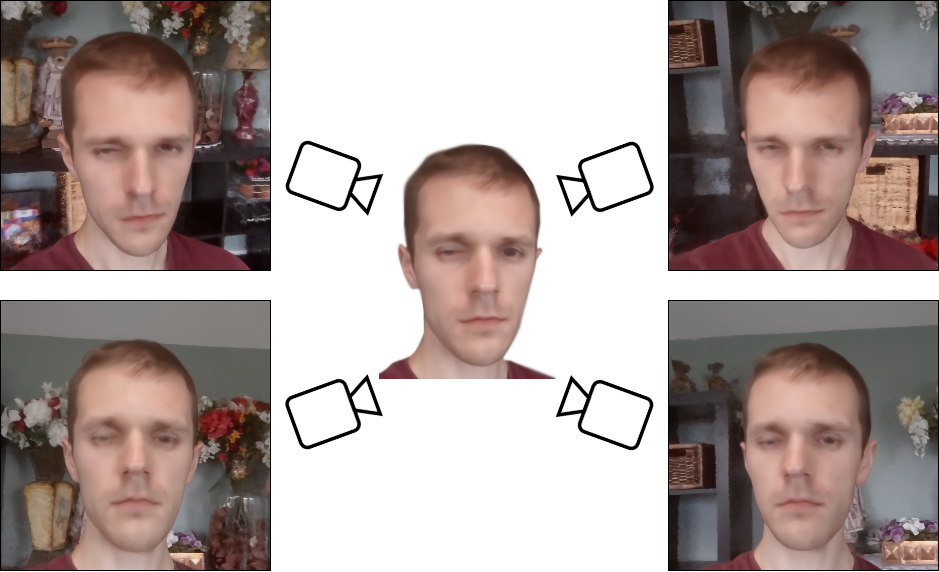
\includegraphics[width=\linewidth]{fig/\conerfdirname/assets/teaser/central.png}
    \subcaption{novel views}
  \end{subfigure}
  \hfill{}
  \begin{subfigure}[b]{0.374\linewidth}
    \centering
    \includegraphics[width=\linewidth]{fig/\conerfdirname/assets/teaser/attributes.pdf}
    \subcaption{novel attributes}
  \end{subfigure}
  \endgroup
}

\fboxsep=0pt % padding thickness
\fboxrule=0.4pt % border thickness
\newcommand{\conerfteaserfigure}{
  \begin{figure}
    \centering
    \teasernobox
    \caption{
      {\bf Teaser --}
      We train a controllable neural radiance field from multiple views of a
      dynamic 3D scene, under varying poses and attributes; in this example
      eye being open/closed and mouth smiling/frowning.
      Given only six annotations (a), our method provides full control over
      the scene appearance, allowing us to synthesize (b) novel views and (c)
      novel attributes, including attribute combinations that were
      \textit{never seen} in the training data~(green box).
    }
    \label{fig:conerf-teaser}
  \end{figure}

}

